\documentclass[UTF8]{ctexart}

\usepackage{subfiles}  

%下面的语句, 引入你的头部设置文件
\usepackage{C:/phpStorm_proj/02_myself_ID_EGO/+100_latex_all_math_sel/myPreamble} 
%必须是绝对路径,才能让各个tex在单独编译时使用到

\title{文件名}


%---------------------------------


\begin{document}
	\tableofcontents % 生成目录
	\date{} % 若不写这句, 则默认也会渲染出日期, 所以我们要手动赋空值
	\maketitle  %这行代码, 让你前面的 title, author, date生效
	
	
	
	\part{条件概率}
	
	\section{``条件概率"的意思}
	
	条件概率是: 有A, B 两个事件, 和样本空间 Ω. 其中 $P(B) >0$, 则, 在B已经发生的条件下, A发生的概率, 就叫做A对B 的``条件概率". 记作:  P(A| 条件B), 读作``在B发生的条件下, A发生的概率”. \\
	
	即, 条件概率公式是: $
	\text{P}\left( \text{A|\ 条件B} \right) =\dfrac{\overset{\text{这个分子即:\ AB同时发生了}}{\overbrace{\text{在B发生条件下,A发生的样本点数}}}}{\text{B里面有多少个样本点}}=\dfrac{\text{n}_{\text{AB}}}{\text{n}_{\text{B}}}
	$ \\
	
	还可写成:  $
	\text{P}\left( \text{A|\ 条件B} \right) 
	=\dfrac{\text{P}\left( \text{A}\cap \text{B} \right)}{\text{P}\left( \text{B} \right)}
	=\dfrac{\frac{\text{n}_{\text{AB}}}{\text{n}}}{\dfrac{\text{n}_{\text{B}}}{\text{n}}}=\dfrac{\text{n}_{\text{AB}}}{\text{n}_{\text{B}}}
		$ \\
	
	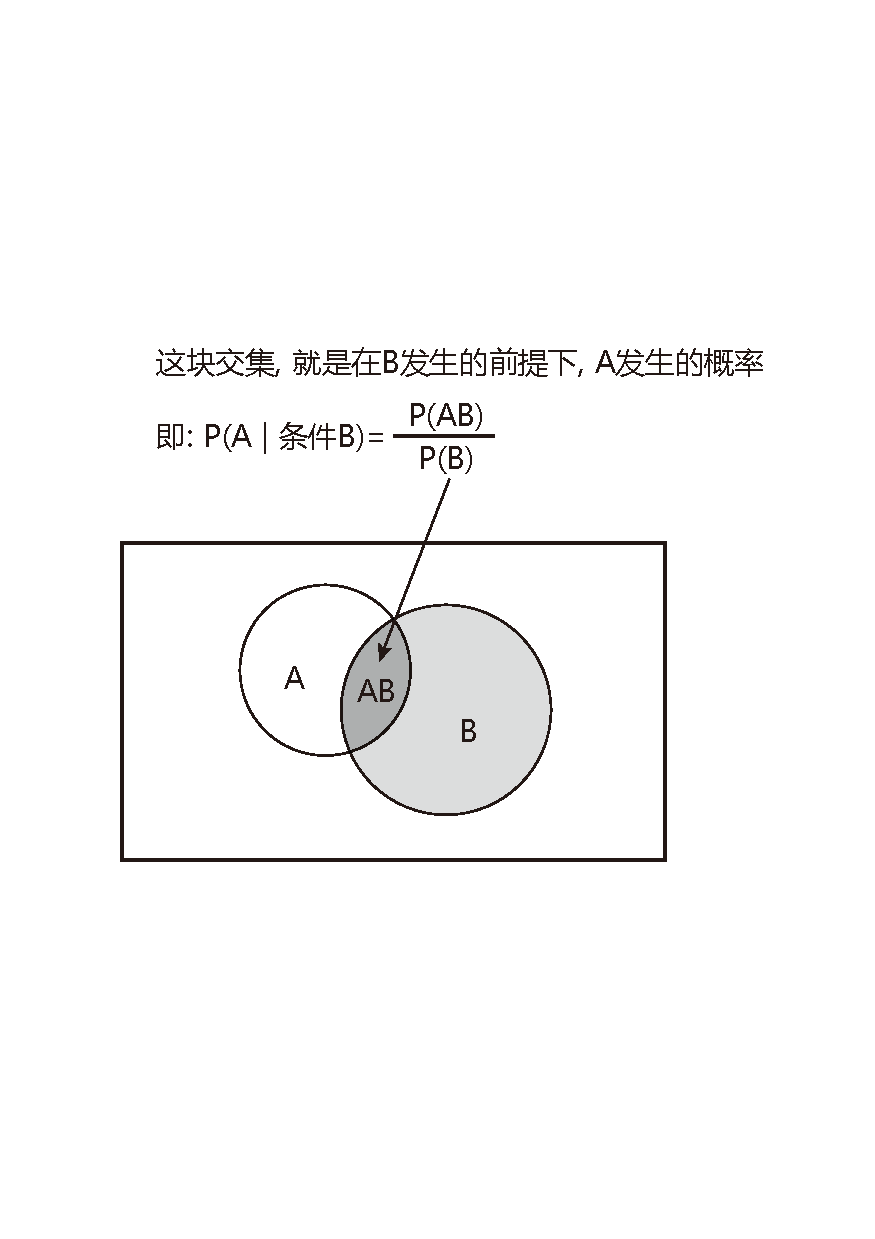
\includegraphics[width=0.5\textwidth]{/0088.pdf} \\
	
	如上图所示, 注意: 概率是个比值, 所以你光有分子那块的交集值, 是没用的, 它还需要与另一个数(分母)去比. \\
	
	\begin{myEnvSample}
		有6个球, 各有编号.  我们先定义下这些事件: \\
		- B: 取到偶数编号的球 \\
		- $A_1$: 取到1号球 \\
		- $A_2$: 取到2号球 \\
		- $A_5$: 取到大于4号的球 \\
		
		则: \\
		- $
		\overset{\text{取到1号球的概率}}{\overbrace{\text{P(A}_1\text{)}}}=\frac{\overset{1\text{号球选}1}{\overbrace{\text{C}_{1}^{1}}}}{\underset{\text{全6选}1}{\underbrace{\text{C}_{6}^{1}}}}=\frac{1}{6}=0.166667
		$
		
		- $
		\text{P}\left( \text{A}_1|\text{B} \right) =\frac{\text{在B条件里面,取到A}_1\text{(即1号球)}}{\text{B:\ 取到偶数编号的球}}=\frac{\overset{\text{偶数编号的球里面,\ 取不到奇数编号的球}}{\overbrace{0}}}{\underset{3\text{个偶数球里面取1个}}{\underbrace{\text{C}_{3}^{1}}}}=0
		$
		
		- $
		\text{P}\left( \text{A}_2|\text{B} \right) =\frac{\overset{1\text{个编号2的球里面,取1个}}{\overbrace{\text{C}_{1}^{1}}}}{\underset{3\text{个偶数球里面取1个}}{\underbrace{\text{C}_{6}^{3}}}}=\frac{1}{3}
		$
		
		- $
		\text{P}\left( \text{A}_5|\text{B} \right) =\frac{\text{在B条件里面,取到大于4号的球}}{\text{B:\ 取到偶数编号的球}}=\frac{\overset{5,6\text{号与偶数的交集,\ 只有6号一个球}}{\overbrace{1}}}{3}
		$
			
	\end{myEnvSample}
	
	
	~\\
	\hrule
	~\\
	
	
	\section{条件概率的性质}
	
	\subsection{性质: $ P(A | \text{条件}B) >= 0$}
	
	
	\subsection{性质: $ P(\Omega | \text{条件}B) = 1$}
	
	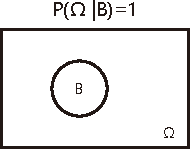
\includegraphics[width=0.25\textwidth]{/0089.pdf}
	
	
	\subsection{性质: $ \text{P}\left( \text{A}_1\cup \text{A}_2\ |\text{B} \right) =\text{P}\left( \text{A}_1\ |\text{B} \right) +\text{P}\left( \text{A}_2\ |\text{B} \right) -\text{P}\left( \text{A}_1\text{A}_2\ |\text{B} \right) 		$}
	
	\subsection{性质: $	\text{P}\left( \text{A\ |B} \right) =1-\text{P}\left( \overline{\text{A}}\ |\text{B} \right) 	$}
	
	\subsection{性质: 可列可加性:  若$ A_1, A_2, ... A_n, ...$ 是``互不相容"的事件, 则有: $ P(\sum_{i=1}^\infty A_i | B) = \sum_{i=1}^ \infty P(A_i | B)$ ← 即: ``和的概率", 等于``概率的和"}
	
	
	
	
	~\\
	\hrule
	~\\
	
	
	\section{乘法公式 : $ P(\text{前后})=P(\text{后}) \cdot P(\text{前}|\text{\text{后}}) = P(\text{\text{前}}) \cdot P(\text{后}|\text{前})$  ← 规律就是``前后前后"这样交错, 或反过来交错.}

	推导过程: \\
	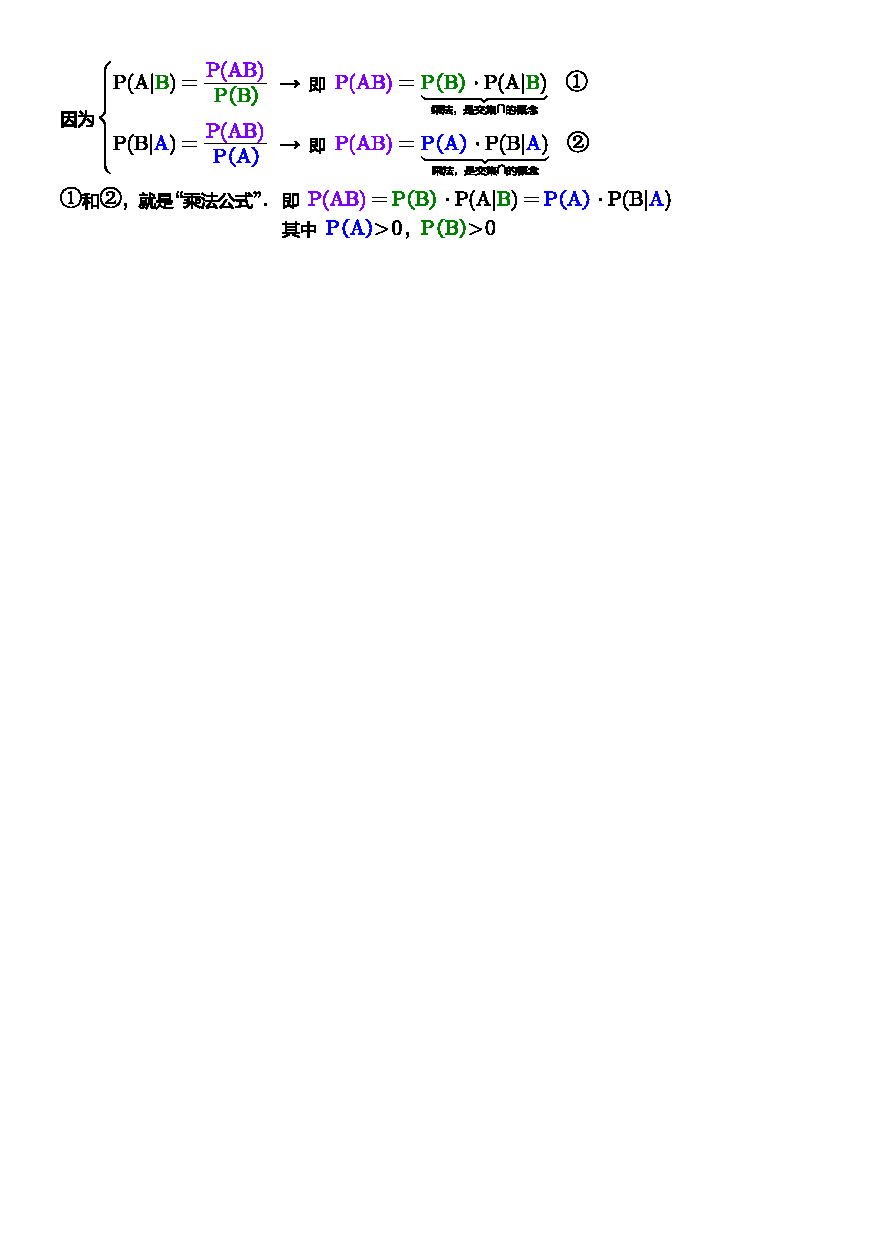
\includegraphics[width=0.8\textwidth]{/0090.pdf} \\
	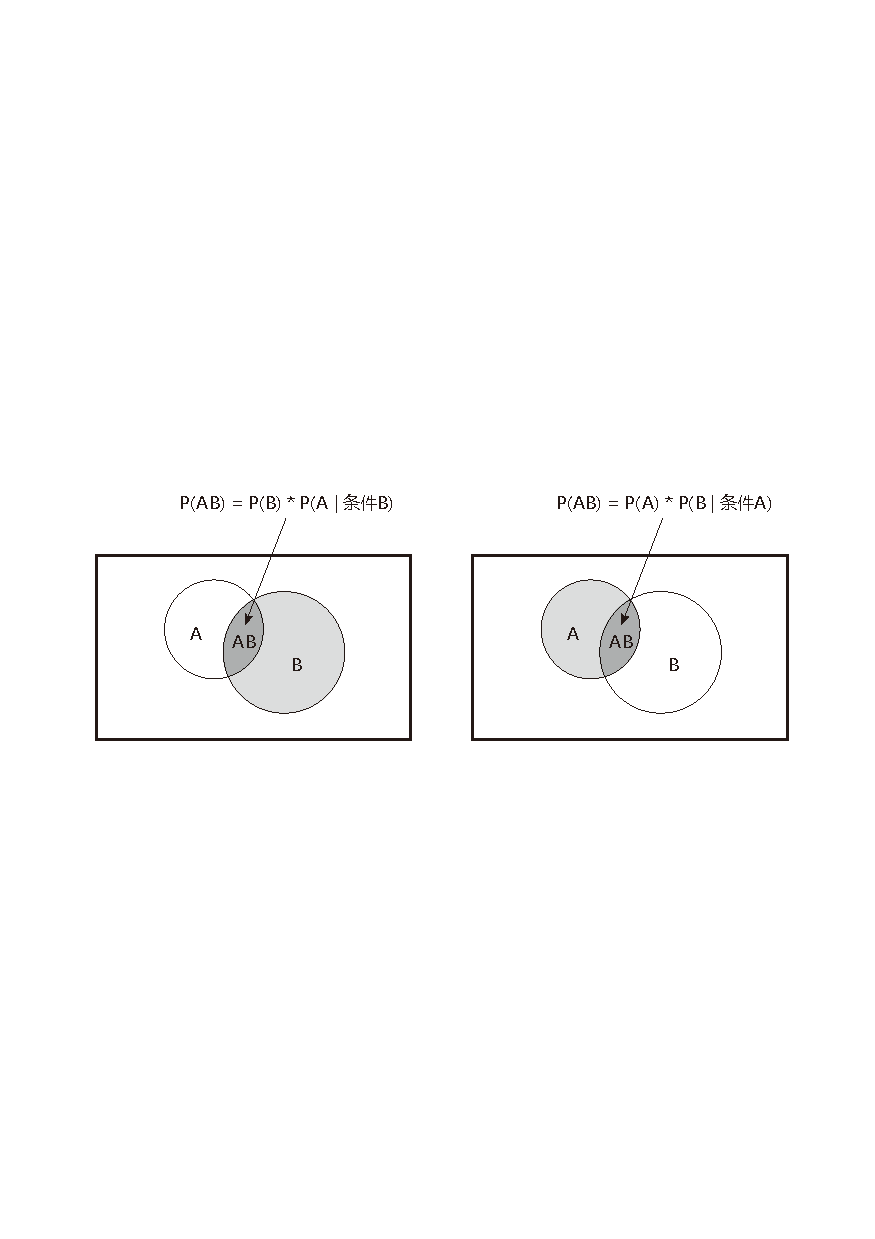
\includegraphics[width=0.8\textwidth]{/0091.pdf} \\
	
	同理, 多个事件的乘法公式就是:  \\
	$ \boxed{
	\text{P(ABC)}=\underbrace{\text{P(A)}}\cdot \underbrace{\text{P(B|A)}}\cdot \underbrace{\text{P(C|BA)}} 	
	}
	$ \\
	↑ 上面``从右往左"看, 就是按 A,B,C 的顺序 \\
	
	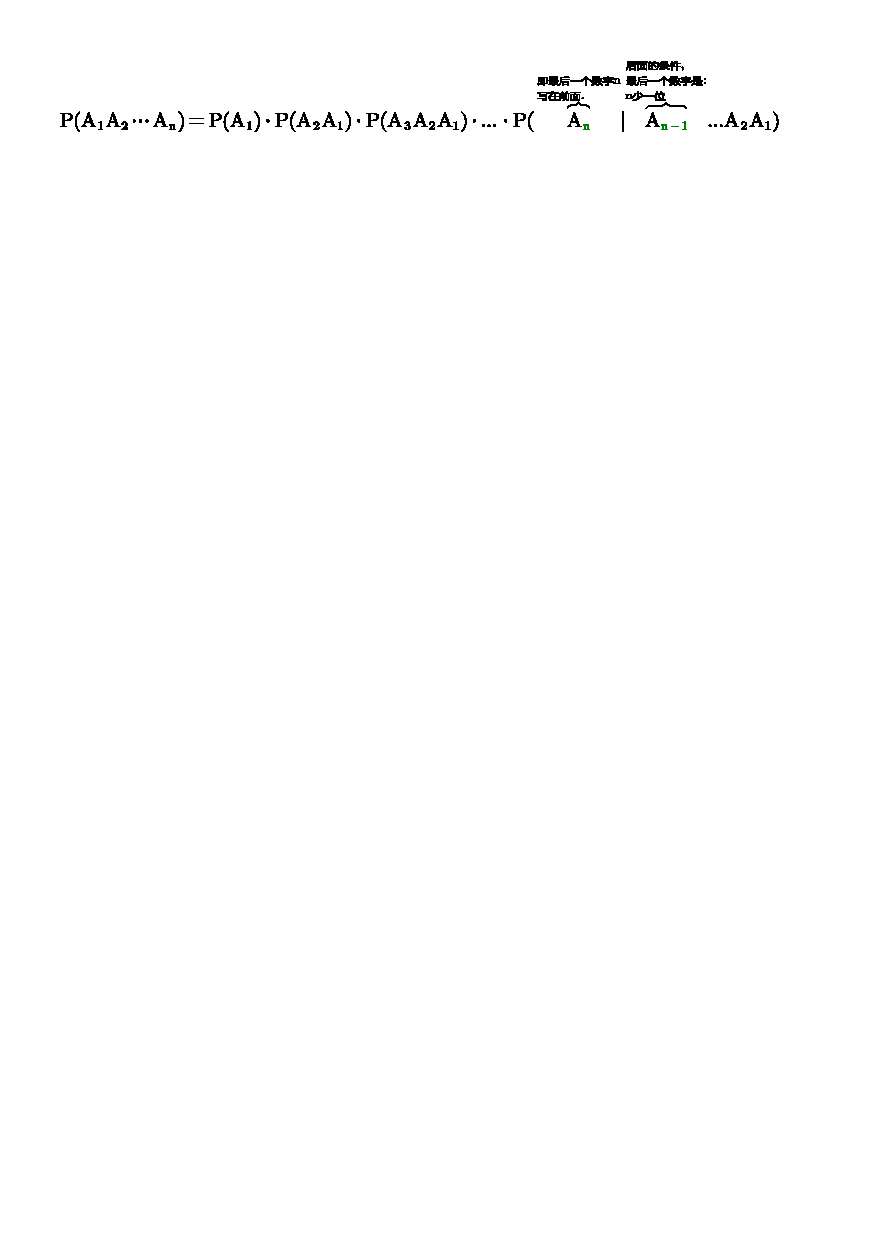
\includegraphics[width=0.95\textwidth]{/0092.pdf} \\
	↑ 上面``从右往左"看, 就是按$A_1, A_2, ... , A_n$的顺序 \\
	
	









	
\end{document}